\documentclass{article}

\usepackage[utf8]{inputenc}
\usepackage[T1]{fontenc}
\usepackage{fourier}
%\usepackage[latin1]{inputenc}
\usepackage[spanish]{babel}

\usepackage[thinlines]{easytable}
\usepackage{diagbox}
\usepackage{multirow}


\usepackage[protrusion=true,expansion=true]{microtype}	
\usepackage{amsmath,amsfonts,amsthm} % Math packages
\usepackage{amssymb}
\usepackage[pdftex]{graphicx}	
\usepackage{url}
\usepackage{tikz}
\usepackage{setspace}
\usepackage{import}
\usepackage{float}
\usepackage{graphicx}
\pagenumbering{arabic}
%margenes 
\usepackage{geometry}
 \geometry{
 a4paper,
 left=19mm,
 right=19mm,
 top=19mm,
 bottom=42mm,
 }

% %%% Custom sectioning
\usepackage{sectsty}
%\allsectionsfont{\normalfont \scshape}


%%% Custom headers/footers (fancyhdr package)
\usepackage{fancyhdr}
\pagestyle{fancyplain}
\fancyhead{}											% No page header
\fancyfoot[L]{}											% Empty 
\fancyfoot[C]{}											% Empty
\fancyfoot[R]{\thepage}									% Pagenumbering
\renewcommand{\headrulewidth}{0pt}			% Remove header underlines
\renewcommand{\footrulewidth}{0pt}				% Remove footer underlines
\setlength{\headheight}{13.6pt}


%%% Equation and float numbering
\numberwithin{equation}{section}		% Equationnumbering: section.eq#
\numberwithin{figure}{section}			% Figurenumbering: section.fig#
\numberwithin{table}{section}				% Tablenumbering: section.tab#


%%% Maketitle metadata
\newcommand{\horrule}[1]{\rule{\linewidth}{#1}} 	% Horizontal rule

\begin{document}

\onehalfspacing

\begin{titlepage}
    
\newcommand{\HRule}{\rule{\linewidth}{0.5mm}} % Defines a new command for the horizontal lines, change thickness here
    
\center % Center everything on the page
     
%----------------------------------------------------------------------------------------
%	HEADING SECTIONS
%----------------------------------------------------------------------------------------
    
\textsc{\LARGE Instituto Tecnológico de Buenos Aires}\\[2cm] % Name of your university/college
\textsc{\Large 22.42 Laboratorio de Electrónica}\\[1.5cm] % Major heading such as course name
\textsc{\large Trabajo Práctico N° 2}\\[0.5cm] % Minor heading such as course title
    
%----------------------------------------------------------------------------------------
%	TITLE SECTION
%----------------------------------------------------------------------------------------
    
\HRule \\[0.5cm]
{ \huge \bfseries Osciloscopios/ Analizador de Impedancias/ \\Circuitos RLC}\\[0.4cm] % Title of your document
\HRule \\[2cm]
     
%----------------------------------------------------------------------------------------
%	AUTHOR SECTION
%----------------------------------------------------------------------------------------
    
\begin{minipage}{0.4\textwidth}
\begin{flushleft} \large
\emph{Grupo 5:}\\		%names
[.3cm]
Nicolás \textsc{De León}\\
Leg. 57232\\ 
[.3cm]
Tomás \textsc{Vigón}\\
Leg. 57327\\ 
[.3cm]
Benjamín \textsc{Lin}\\
Leg. 57242 \\ 
[.3cm]
Lucero Guadalupe \textsc{Fernandez}\\
Leg. 57485\\ 
[.3cm]
\end{flushleft}
\end{minipage}
~
\begin{minipage}{0.4\textwidth}
\begin{flushright} \large
\emph{Profesor:} \\
[.3cm]
Pablo  \textsc{Cossutta}\\ % Supervisor's Name
Alejandra \textsc{Weill} \\% Supervisor's Name
Matías  \textsc{Salvati} % Supervisor's Name
\end{flushright}
\end{minipage}\\[2cm]
    
%----------------------------------------------------------------------------------------
%	DATE SECTION
%----------------------------------------------------------------------------------------
    
\vfill
{\large Entregado: 25 de Septiembre de 2018}\\[2cm]
    
\vfill 
    
\end{titlepage}

\section{Medición de Componentes Pasivos con Analizador de Impedancias}
\subsection{Inductor}
Utilizando el analizador de impedancias se midió el valor de L, su factor de calidad Q, y la resistencia de una bobina de 1mH, entre 10Hz y 10MHz.
Se propuso el siguiente modelo eléctrico equivalente:

\begin{figure}[h!]
\centering
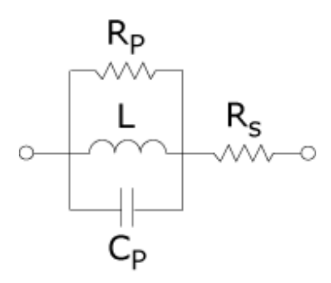
\includegraphics[scale=0.5]{modeloL.png}
\caption{Modelo eléctrico equivalente de la bobina}
\label{fig:modeloL}
\end{figure}

Se calculó la impedancia equivalente del modelo como:

\begin{equation}
Z_L=\frac{\omega^2L^2R_p}{(R_p-\omega^2C_pR_pL)^2+(\omega L)^2}+R_s+j\frac{(\omega LR_p)(R_p-\omega^2 CLR_p)}{(R_p-\omega^2C_pR_pL)^2+(\omega L)^2}
\end{equation}
En este modelo, $C_p$  representa la capacitancia parásita presente entre las espiras de la bobina, a su vez, $R_s$ y $R_p$, las pérdidas en el cobre y en el material magnético, respectivamente.
Para hallar los valores de los componentes, se analiza de las mediciones la frecuencia de resonancia, que es cuando la impedancia es real, es decir, su fase es $0^o$. Esta se encuentra alrededor de los 1,8MHz.
Igualando la parte imaginaria y evaluando en la frecuencia de resonancia se encuentra que $C_p=\frac{1}{4\pi^2f^2L}=7.82pF$. Con ésto, se aproximaron los valores de $R_s$ y $R_p$ que mejor se asemejaban a la curva medida respecto a la teórica. Partiendo de que, mientras $R_s$ debía ser un valor chico, $R_p$ debía ser un valor grande, para no disminuir los efectos inductivos de la bobina, se llegó a $R_s=1\Omega$ y $R_p=5M\Omega$.

\begin{figure}[h!]
\centering
\includegraphics[scale=0.5]{bodeL.png}
\caption{Impedancia de la bobina de 1mH.}
\label{fig:bodeL}
\end{figure}

Por otro lado, también se graficaron las curvas de la resistencia R y la inductancia L de la bobina aproximando la curva de impedancia.

\begin{figure}[h!]
\centering
\includegraphics[scale=0.5]{RdelL.png}
\caption{Resistencia del inductor.}
\label{fig:RdelL}
\end{figure}

\begin{figure}[h!]
\centering
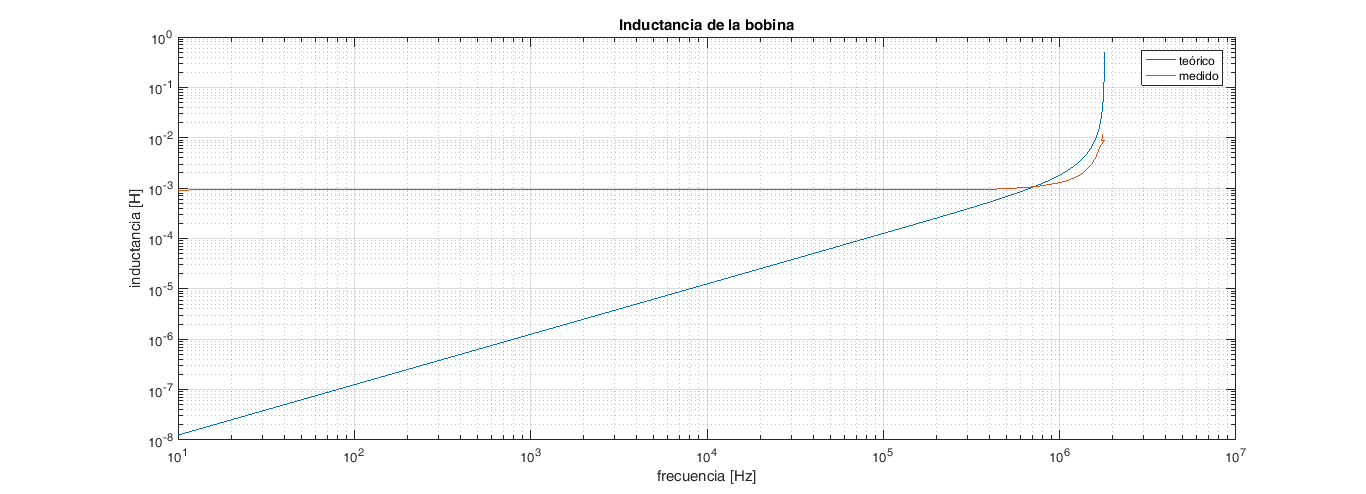
\includegraphics[scale=0.5]{LdelL.png}
\caption{Inductancia de la bobina.}
\label{fig:LdelL}
\end{figure}

Puede verse que los valores de inductancia y resistencia del modelo difieren de los medidos en el analizador, siendo la inductancia del equivalente mayor a la medida, y la resistencia lo contrario, es decir, la teórica resulta menor a la medición.  Esto puede deberse a que los valores de los componentes resistivos del modelo se aproximaron con la curva de la impedancia, y no con las curvas de la resistencia/inductancia.
Estos errores son también apreciables al graficar la curva del factor de calidad de la bobina ($Q=\frac{X_L}{ESR}$). A pesar de que las formas de las curvas son iguales, los errores arrastrados en la resistencia e inductancia afectan notoriamente a la curva del Q.

\begin{figure}[h!]
\centering
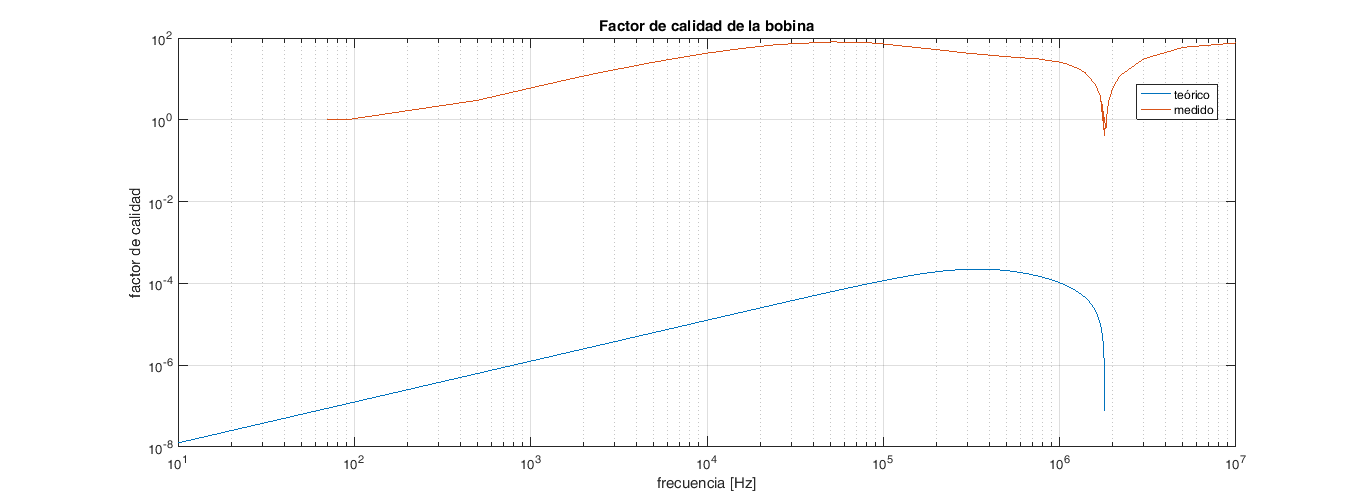
\includegraphics[scale=0.5]{QdelL.png}
\caption{Factor de calidad de la bobina.}
\label{fig:QdelL}
\end{figure}

\section{Respuesta del Circuito LRC}

Se armo el circuito LRC representado en la figura \ref{fig:LRC2}, cuyos valores nominales son $L=1mH$ para la bobina y $C=8.2nF$ para el capacitor. Con el uso de un Buffer en la entrada se evitar impedancia del generador y que se cargue el generador, provocando un funcionamiento incorrecto durante las mediciones.

\begin{figure}[h!]
\centering
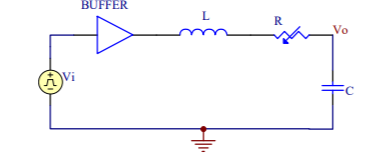
\includegraphics[scale=0.5]{lrcCircuito.png}
\caption{Circuito LRC armado}
\label{fig:LRC2}
\end{figure}

La ecuacion característica del circuito es $\frac{s^2}{\omega_0^2}+s\frac{2\xi}{\omega_0}+1$, donde $\omega_0 = \frac{1}{\sqrt{LC}}$ y $\xi = \frac{\omega_0RC}{2}$. Calculado la frecuencia de resonancia $f_0=55.5kHz$ y teniendo en cuenta el valor de $\xi = 0.19$ hallamos el valor de la resistencia $R = 130\Omega$. Cabe notar que el factor de calidad $Q = \frac{1}{2\xi}$ por lo que resulta en este caso $Q = 2.6$, por lo tanto se trataria de un circuito sub-amortiguado. 

\subsection{Respuesta al Escalon}

Exitando el circuito con una onda cuadrada de $V_i = 0.5V_{pp}$ y una frecuencia de $f = 5.5kHz$ obteniendo la siguiente respuesta:

\begin{figure}[h!]
\centering
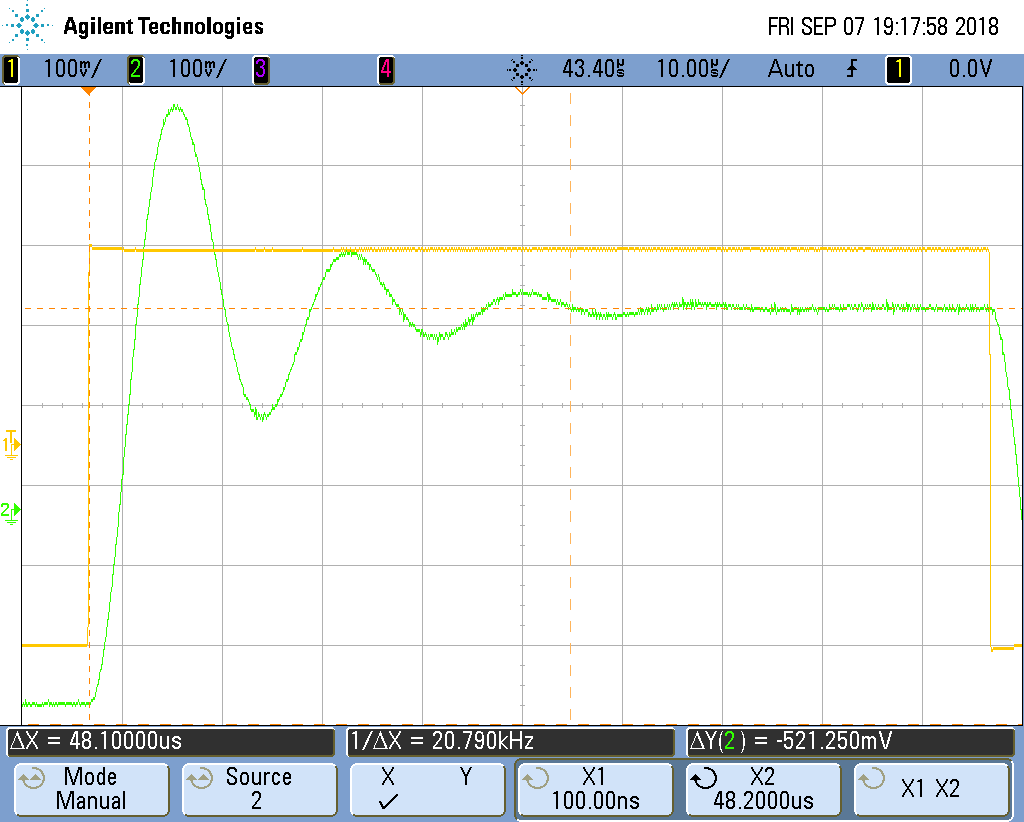
\includegraphics[scale=0.25]{LRC2a.png}
\caption{Respuesta al escalon}
\label{fig:LRC2a}
\end{figure}

De tal manera que se obtuvo un sobrepico de $S_p = 257mV$, un tiempo de establecimiento del $5\%$ $t_s = 47.6{\mu}s$ y su frecuencia de oscilacion $f_t = 56.2kHz$. Como criterio para la medicion del tiempo de establecimie se tomo la diferencia de tiempo desde la exitacion de la señal cuadrada y el tercer sobrepico de la oscilacion. Notamos que la señal de salida tiene comportamiento de una oscilacion subamortiguada, donde el capacitor y la inductancia en seria actuan como un oscilador y la resistencia actua como dicipador de energia reduciendo asi la amplitud de la oscilacion.

Se obtuvo la respuesta analitica del circuito partiendo de la ecuacion: $$\frac{V_c''(t)}{\omega_0^2} + \frac{V_c'(t) 2\xi}{\omega_0} + V_c(t) =  0.5u(t)$$ tal que las condiciones iniciales son nulas. Con el uso de la transformada de Laplace llegamos a $V_c(s) = \frac{0.5}{s(\frac{s^2}{\omega_0^2}+\frac{s2\xi}{\omega_0}+1)}$ por lo que su antitransformada es equivalente a:$$V_c(t) = 0.5\left(1-\frac{e^{-\xi\omega_0t}}{\sqrt{1-\xi^2}}\sin{\left(\omega_0\sqrt{1-\xi^2}t+\arctg{\frac{\sqrt{{1-\xi^2}}}{\xi}}\right)}\right)$$ 
De esta manera se podra derivar $V_c(t)$ y hallar el punto critico, es decir el sobrepico de la funcion que tiene forma $t_p=\frac{\pi}{\omega_0\sqrt{1-\xi^2}}$, lo que resulta en este caso $t_p=9.18{\mu}s$ y su correspondiente valor $S_p=0.5\left(e^{\frac{-\xi\pi}{\sqrt{1-\xi^2}}}\right) =272mV$. Como describe la ecuacion la frecuencia de oscilación es $f_t= \frac{\omega_0\sqrt{1-\xi^2}}{2\pi} = 54.5kHz$. Por ultimo el tiempo de establecimiento de la señal la aproximamos con $t_s=\frac{\pi}{\xi\omega_0}$ que obtenemos $t_s = 47.42{\mu}s$

Comparando los resultados analiticos y experimentales, los resultados estan en el mismo orden si bien existen diferencias las cuales pueden ser debido a errores accidentales en las mediciones y aproximaciones en los calculos teoricos. 

\subsection{Effecto de la frecuencia en el circuito LRC}

Con el uso del del circuito anterior se observo la onda de salida exitada con una señal cuadrada de duty $50\%$ variando su frecuencia partiendo de $f_i=5.5kHz$.

Inicialmente, como las condiciones eran identicas a la experiencia anterior se vio en la señal su correspondiente periodo transitorioy su periodo estacionario en cada escalon. Sin embargo al aumentar la frecuencia, disminuye la cantidad de periodos de oscilaciones en la respuesta del escalon del circuito. 

Al llegar a la frecuencia de resonancia $f_0$ la señal de salida oscila en transitorio y tiene forma de una senoidal como la frecuenciade la señal cuadrada es similar a su frecuencia de la oscilación $f_t$, por lo que siendo el duty cycle de la función de entrada $50\%$, solo medio período de la oscilacióno ocurre antes de que se presente un nuevo escalón de tensión, es decir notamos un solo maximo en cada escalon. Aumentando la frecuencia desde este punto, la forma de la onda es identica a la de $f_0$, pero la amplitud de la señal de salida se ve atenuada. Podemos explicar este fenomeno ya que el circuito tiene cracteristica de un pasa bajos el cual las altas frecuencias son filtradas y solo deja el paso de frecuencias bajas. 

\subsection{Diagrama de Bode}

Realizando un barrido de frecuencia entre $\frac{f_0}{10}$ a $20f_0$ con una onda senoidal, se midio la amplitud y la fase de tension del capacitor. Con el uso de los datos obtenidos se realizo su correspondiente diagrama de Bode. Ademas, se calculo la respuesta en transferencia del circuito que tiene la forma $H(s)=\frac{1}{s^2LC+sRC+1}$ con los valores de L, C y R los valores mencionados previamente.

\begin{figure}[h!]
\centering
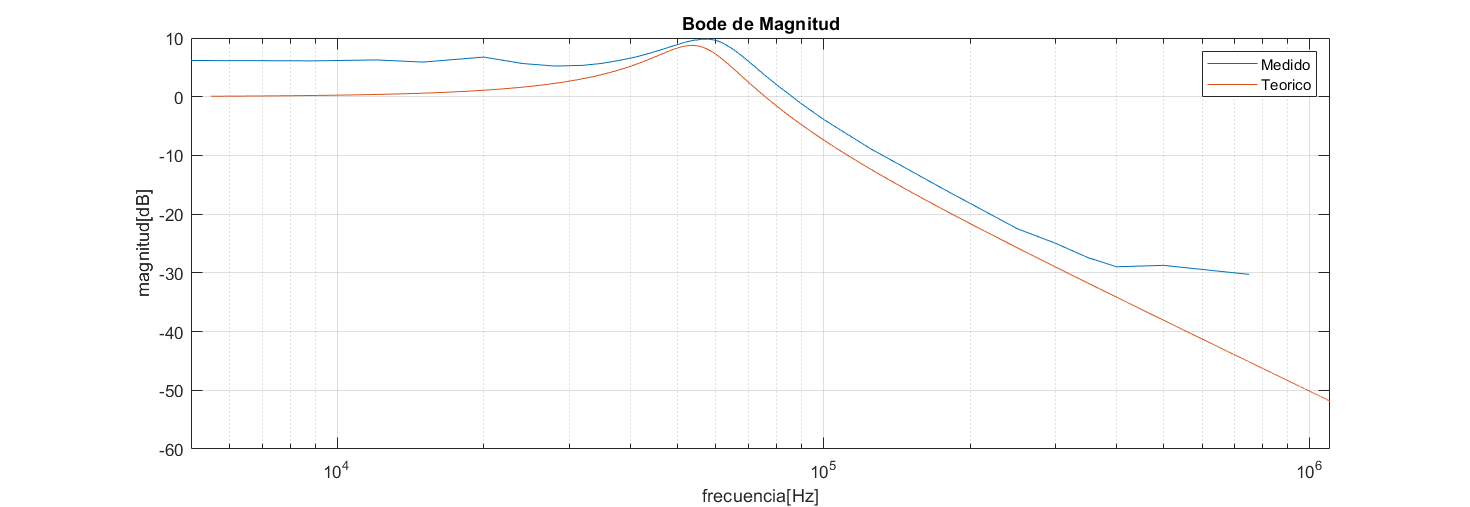
\includegraphics[scale=0.25]{2cmag.png}
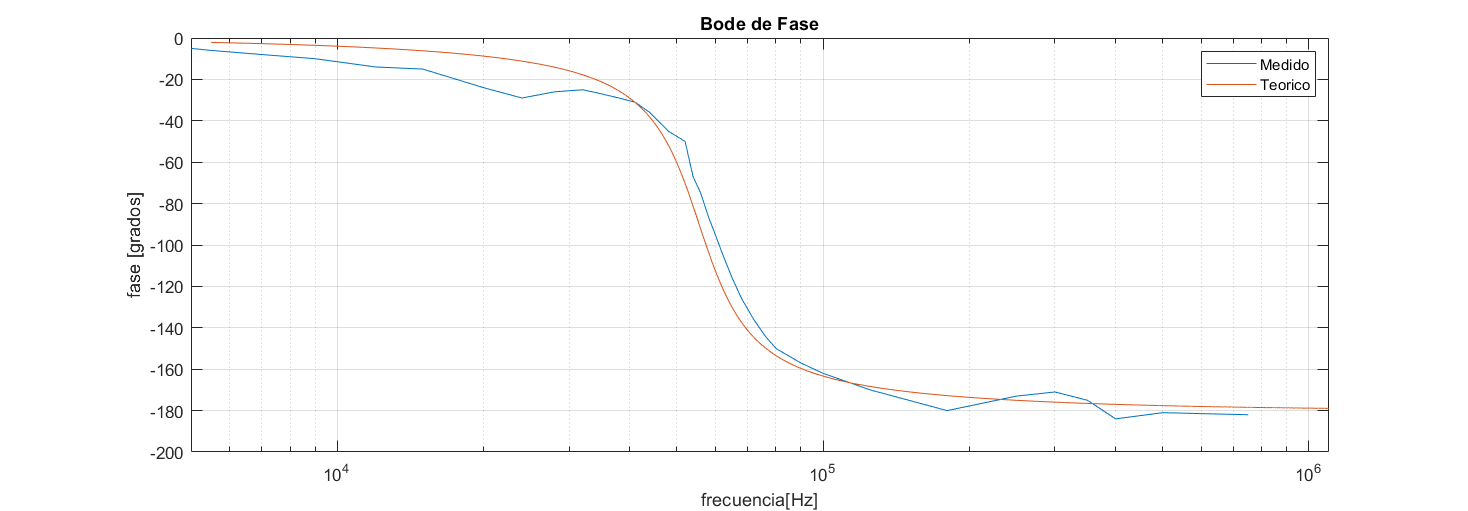
\includegraphics[scale=0.25]{2cfase.png}
\caption{Diagrama de Bode}
\label{fig:LRC2c}
\end{figure}

\pagebreak

De la figura \ref{fig:LRC2c} identificamos que el circuito de segundo orden actua como un filtro pasa bajos y tiene su respectivo sobrepico al rededor de $f_p=f_0\sqrt{1-2\xi^2}=53.5kHz$. Analizando el Bode con el punto anterior, reconocemos que a frecuencias mayores a $f_0$ la salida es atenuada respecto a la entrada como tambien la frecuencia en que la amlitud maxima del sobrepico de la salida coincide con el la frecuencia $f_p$, al rededor de la $f_0$

Si bien identificamos diferencias en el Bode medido y el Bode teorico, a grandes razgos son identicas. Estas diferencias pueden ser debido a la tolerancia de los componentes utilizado y errores accidentales en las mediciones de las mismas. 

\subsection{Respuesta al escalon condicionadas}

\subsubsection{Sobrepico de $\bold{0,2V}$} \label{dSobrepico de 0.2v}

En primera instancia se busco el valor de R experimentalmente tal que el sobrepico sea de $S_p=0.2V$. Variando su valor se hallo que la resistencia que cumple tal condicion es $R=184\Omega$. En estas condiciones su frecuencia de oscilacion $f_t=56.8kHz$ y su tiempo de establecimiento $t_s = 44.1{\mu}s$. 

\begin{figure}[h!]
\centering
\includegraphics[scale=0.075]{2d1.jpg}
\caption{Sobrepico de $0.2V$}
\label{fig:LRC2d1}
\end{figure}

Sin embargo analiticamente con tal valor de R, el valor de sobrepico es $S_p = 214mV$, $f_t= 53.6kHz$ y $t_s = 47.4{\mu}s$. Estos resultados pueden variar con el experimental debido a la tolerancia y a errores de apreciacion al medir el sobrepico. Por ello tambien se hallo la resistencia teorica que daria el sobrepico de $0.2V$, la cual remplazando en la ecuacion de sobrepico el $\xi=0.28$ por lo tanto $R=180\Omega$, donde la diferencia de valor de R puede atribuirse a errores accidentale en la medicion y no tener encuenta la tolerancia de los componentes. 

\subsubsection{Resistencia de $\bold{18k\Omega}$}

Remplazando la resistencia con uno de valor $R=18k\Omega$, lo que es $100$ veces la resistecia del item anterior observamos lo siguiente:

\begin{figure}[h!]
\centering
\includegraphics[scale=0.075]{2d2.jpg}
\caption{Respuesta del Circuito con Resistencia de $18k\Omega$} 	
\label{fig:LRC2d2}
\end{figure}

De la figura \ref{fig:LRC2d2} notamos que el circuito es atenuado y no llega a su periodo estacionario. Este fenomeno puede atribuirse a que el incremento de la resistencia provoca un incremento en el tiempo de carga en el capacitor; el tiempo caracteristico del capacitor es $\tau = RC$ en este caso $\tau = 147{\mu}s$ por lo que cuya velocidad de carga se ve reducido por el incremento del valor de resistencia. Ademas, sabiendo que la señal de cuadrada de duty $50\%$ esta en su estado mas alto tan solo $90.9{\mu}s$, lo que el capacitor no llega a cargarse y descargarse. 

\subsubsection{Sin Resistencia}\label{dsinresistencia}

Retirando la resistencia en el circuito, se espera una señal de salida con forma de una oscilacion armonica teniendo $V_c(t) = 0.5\left(1-\sin{\left(\omega_0t+\frac{\pi}{2}\right)}\right)$. Sin embargo se obtuvo:

\begin{figure}[h!]
\centering
\includegraphics[scale=0.075]{2d3.jpg}
\caption{Respuesta del Circuito sin Resistencia} 	
\label{fig:LRC2d3}
\end{figure}

\pagebreak

En el cual la respuesta siguie teniendo forma de una oscilacion subamortiguada, de $S_p = 562mV$, $f_t = 58.1kHz$ y no llega a establecerse al $5\%$. Por lo que notamos una leve reduccion en la amplitud; esta puede atribuirse a la resistencia de los cables usados y como los C y L utilizados en el circuito no son ideales, entonces precentan resistividad  parasita. Esta resistencia  parasita, si bien pequeña, dicipa energia del sistema en cada oscilacion.

\subsubsection{Circuito Criticamente Amortiguado}

Para que el circuito llegue a su estado de establecimiento lo mas veloz posible, lo que el circuito seria criticamente amortiguado ya que que el tiempo de establecimiento seria el mínimo, existe un $R_c$, donde $\xi = 1$, lo que resuta analiticamente ser $R_c = 700\Omega$. 

\begin{figure}[h!]
\centering
\includegraphics[scale=0.075]{2d4.jpg}
\caption{Respuesta del Circuito con Resistencia de $601\Omega$} 	
\label{fig:LRC2d4}
\end{figure}

A pesar de ser la resistencia teorica de $700\Omega$, experimentalmente el valor de la resistencia usada fue $R = 601\Omega$. Es razonable que el valor de la resistencia disminuya ya que en el circuito existen resistencias parasitas. Tambien es posible que halla errores accidentales durante la medicion y que los componentes presentan tolerancias.

\subsection{Respuesta del Circuito sin Buffer}

\subsubsection{Sobrepico de $\bold{0,2V}$} 

Repitiendo la experiencia del punto \ref{dSobrepico de 0.2v}, pero ahora sin el uso de un Buffer se obtuvo la siguiente respuesta:

\begin{figure}[h!]
\centering
\includegraphics[scale=0.075]{2e1.jpg}
\caption{Sobrepico de $0.2V$ sin Buffer} 	
\label{fig:LRC2e1}
\end{figure}

Utilizando el mismo valor del punto \ref{dSobrepico de 0.2v}, se obtuvo un sobrepico de $S_p = 180mV$, por ello se vario el valor de resistencia, disminuyendola para obtener un sobrepico de $0.2V$. Esto es debido que el Buffer permitia que el circuito sea independiente del generador que tenia impedancia interna de $50\Omega$, al quitarlo la resistencia mencionada comienza a afectar al circuito y ademas es posible que se cargue el generador provocando una leve alteracion en la señal de entrada.

\subsubsection{Sin Resistencia}

Quitando el Buffer y la resistencia del circuito se observo la señal de salida:

\begin{figure}[h!]
\centering
\includegraphics[scale=0.075]{2e3.jpg}
\caption{Sobrepico de $0.2V$ sin Buffer} 	
\label{fig:LRC2e3}
\end{figure}

Como en el punto \ref{dsinresistencia}, no se pudo obtener el tiempo de establecimiento al $5\%$, si bien la oscilacion es mas amortiguada teniendo un $S_p = 0.4V$, ya que la resistencia interna del generador de $50\Omega$no es suficiente como para poder disipar la suficiente cantidad de energia estabilizando la señal. Ademas, notamos que la señal de entrada tambien oscila ya que generador se carga de tal manera que sin una resistencia suficiente no puede disipar la suficiente cantidad de energia para establecerse.

\end{document}
